% !TEX root =  ../technisch.tex
\subsection{Docker}

% PLAGIAT

\textcolor{red}{\textbf{DER TEXT MUSS NOCH PLAGIATSFREI GEMACHT WERDEN!}}

Docker ist eine von dem Unternehmen Docker Inc. entwickelte Software, welche eine Art der Container-Virtualisierung ermöglicht. 
Die Container-Virtualisierung ist eine leichtgewichtige und ressourcenschonende Variante der Virtualisierung von Arbeitsumgebungen für Anwendungen. 
Im Gegensatz zu virtuellen Maschinen bilden Container kein eigenständiges System ab, welches über virtuelle Hardware und ein vollständiges Betriebssystem verfügt. 
Vielmehr stellen sie eine isolierte Umgebung für eine spezifische Anwendung dar, welche die Ressourcen des zugrundeliegenden Systems verwenden. 

\begin{figure}[h]
	\centering
	\captionsetup{justification=centering}
	\subfigure[Container-Virtualisierung]{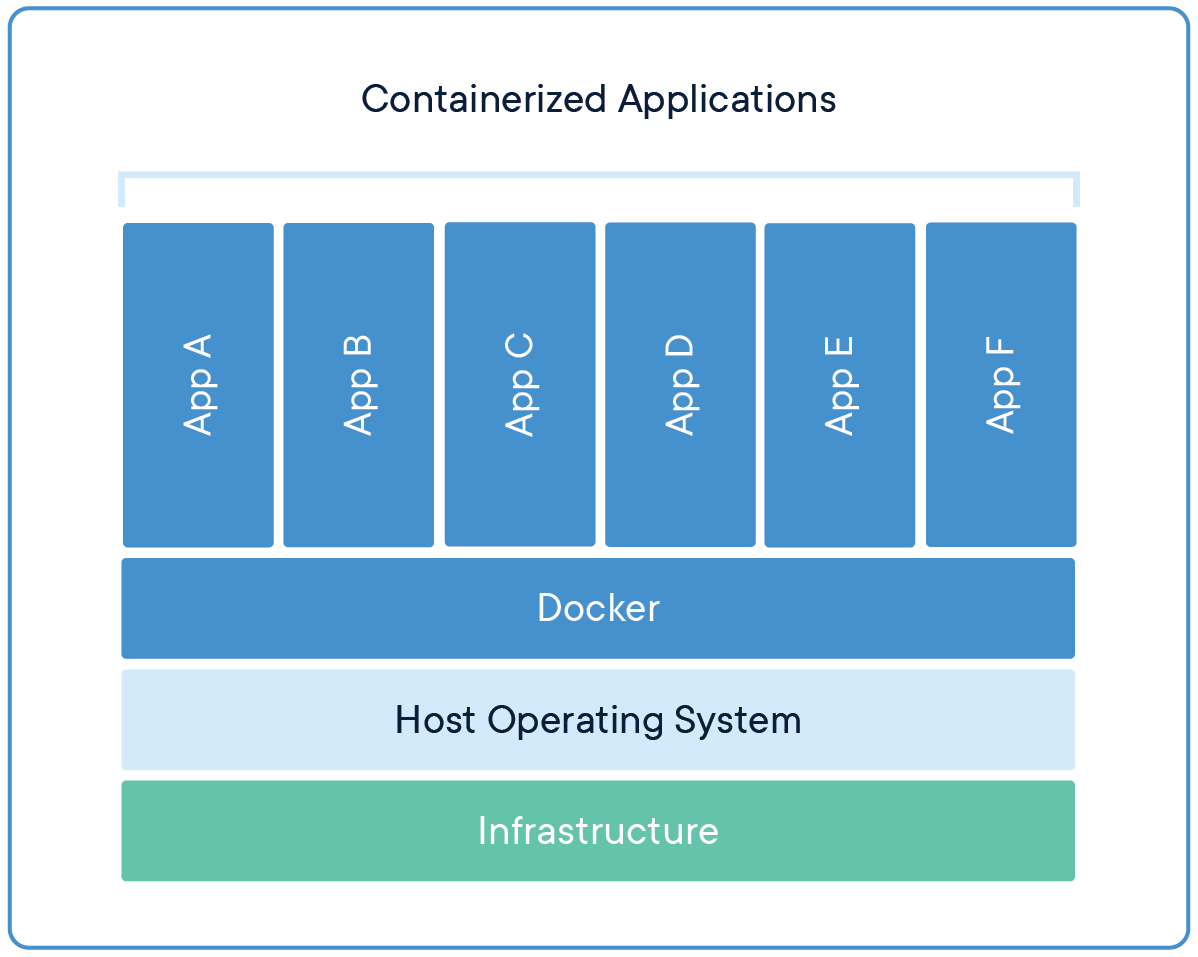
\includegraphics[width=0.45\textwidth]{content/grundlagen/technisch/img/docker_container}}\hspace{1cm}
	\subfigure[Virtuelle Maschine]{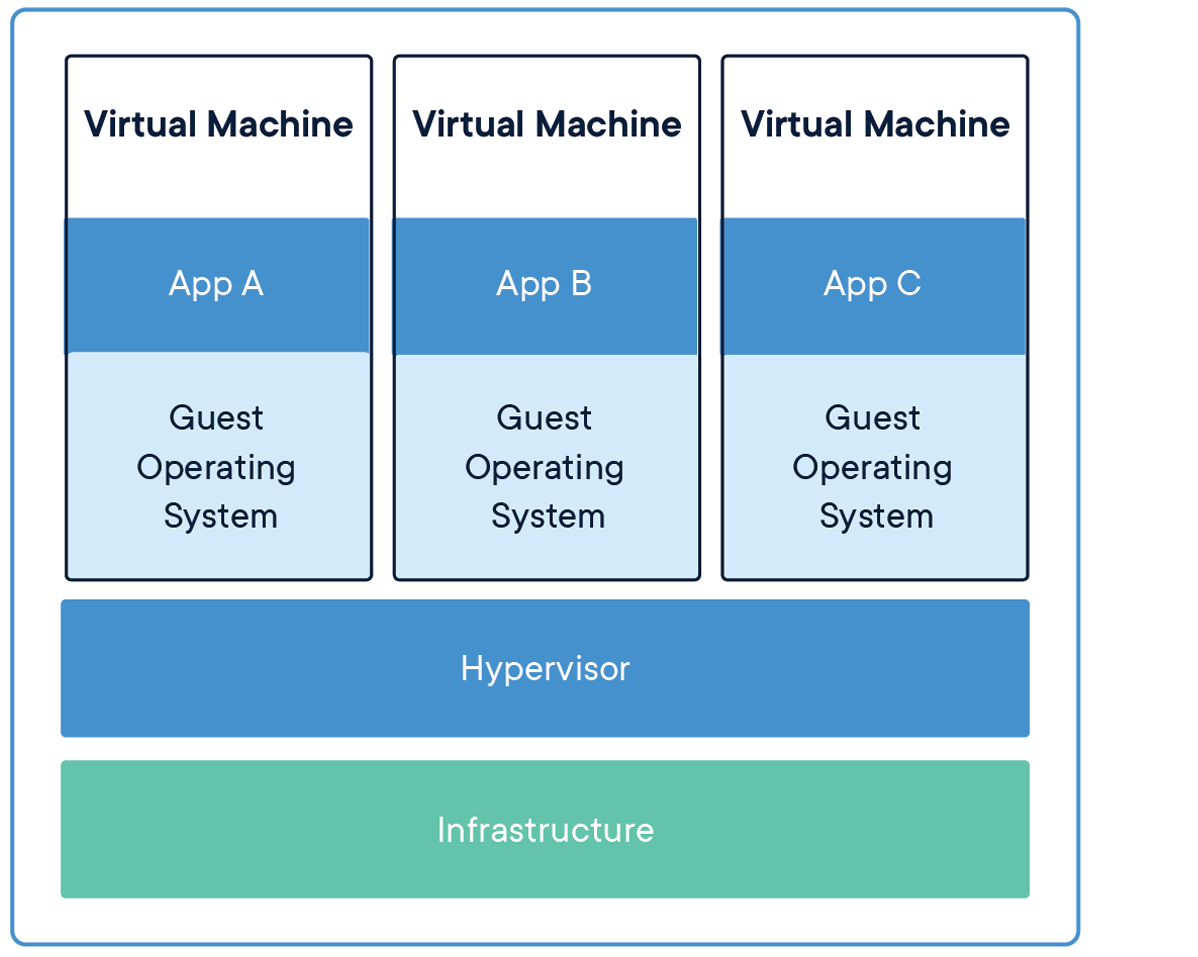
\includegraphics[width=0.45\textwidth]{content/grundlagen/technisch/img/docker_hypervisor}}
	\caption[Vergleich Container-Virtualisierung vs. virtuelle Maschine]{\label{fig:docker_container}Vergleich Container-Virtualisierung vs. virtuelle Maschine, \\Quelle: \cite{MS-DockerInc..05.03.2019}}
\end{figure}

Abbildung \ref{fig:docker_container} verdeutlicht den Aufbau von Container-Virtualisierung und zeigt einen Vergleich zu Hardware-Virtualisierung.\autocite[Vgl.][]{MS-ChrissiKraus.27.07.2018}$^,$\autocite[Vgl.][]{MS-MicrosoftCorporation.31.08.2018} 
Wie man sehen kann, setzt Docker auf dem zugrunde liegenden Betriebssystem auf, wohingegen eine virtuelle Maschine als Gast-System agiert, bei der ein Hypervisor, also ein Manager für virtuelle Maschinen\autocite[Vgl.][]{MS-ReneBust.06.04.2010}, diese verwaltet und die Verteilung der Hardware-Ressourcen übernimmt.

Weitere Vorteile von Docker sind das hohe Maß an Integration und eine gute Skalierbarkeit von Anwendungen. 
Docker-Container lassen sich einfach erzeugen, starten und stoppen. 
Dabei ist die sogenannte Docker-Engine, welche als Kern- und Steuerprogramm von Docker fungiert, dazu in der Lage, die Container zu replizieren bzw. die Anzahl an Containern für einen speziellen Dienst bei Bedarf beliebig zu erhöhen oder zu verringern. 
Die Integration entsteht darin, dass Docker mit anderer Software interagieren bzw. sich von dieser steuern lassen kann.